%!TEX root = ../thesis.tex
\begin{savequote}[75mm]
This is some random quote to start off the chapter.
\qauthor{Firstname lastname}
\end{savequote}

\chapter{Methods}

The Discrete Voter Model is implemented in Python 3, and the accompanying code is found in the repository noted in \hyperref[chap:appendix]{Appendix A}. A set of $5$ modules supports the Discrete Voter Model, with each implementing an aspect of the statistical framework. Those modules are:

\begin{enumerate}
  \item \texttt{phc}: creates probabilistic hypercubes
  \item \texttt{expec\_votes}: finds the expectation of votes for a candidate
  \item \texttt{prob\_votes}: finds the probability of an electoral outcome
  \item \texttt{elect}: aggregates election and electorate data
  \item \texttt{dvm}: executes the Markov chain on a state space of hypercubes
\end{enumerate}

The modules work together to run the Discrete Voter Model on an \texttt{Election} object to generate a distribution of probabilistic hypercubes for the election. Each probabilistic hypercube encodes a probability distribution within a potential precinct of the district, and is used to extract the likely demographic voting probabilities.

These demographic voting probabilities are the goal of the ecological inference, and provide information to answer whether voting in an election is polarized by race.

\section{phc}
\label{sec:phc}

\newthought{The Discrete Voter Model} introduces the probabilistic hypercube (PHC) to represent the distribution of possible demographic voting probabilities in a precinct, for a candidate.

A probabilistic hypercube (PHC) is defined as a rank $n$ tensor (matrix, multidimensional array, or holor) in $\mathbb{R}^n$ space with the following characteristics:
\begin{enumerate}
  \item the component values of the cells sum to $1$
  \item each dimension corresponds to a demographic group in an electorate
  \item each cell's position, or index, represents the demographic voting probabilities of a precinct
  \item each cell's component value represents the inferred probability of that cell representing the true demographic voting probability of a precinct
\end{enumerate}

The function \texttt{make\_phc} initializes a PHC with either random or uniform cell components. The rank of the PHC corresponds to the number of demographic groups being analyzed by the model. The size of each dimension is the \textit{granularity} of the discretization, and thus the model.

For example, a PHC with granularity $100$ meant to represent $3$ demographic groups will have the shape $(100, 100, 100)$, and can be thought of as a $100 \times 100 \times 100$ matrix.

The demographic voting probabilities (DVP), the collection of $b_i$ from King's model specification, are derived for a cell directly from that cell's position within the PHC. The higher a cell is along a dimension of the tensor, the higher the probability that members of that dimension's corresponding demographic group will vote for a candidate.

For example, in a precinct with $2$ demographic groups, and in a PHC with granularity $10$, a cell at the position $10, 0$ represents $\frac{10}{10} = 100 \%$ of demographic group $1$ voting for the candidate, and $\frac{0}{10} = 0 \%$ of demographic group $2$ voting for the candidate.

In general, in some PHC with granularity $d$ representing $n$ demographic groups, for some cell at index $\{i_0, i_1, i_2, \dots, i_n\} = \left\{i_j\right\}_{j=0}^n$:

$$\text{DVP} = \left\{\frac{i_j}{d}\right\}_{j=0}^n$$

When given a precinct, candidate, and some PHC, one can determine the demographic voting probability of the precinct for the candidate by sampling a cell, or set of cells, from the PHC randomly, using the cell's component values as probabilities. The higher the component value of a cell, the more likely it is to be chosen to be the inferred demographic voting probability of the given precinct and candidate.

The granularity of the discretization is directly related to how precise the demographic voting probabilities are. In general, the higher the granularity of a PHC, the more precise its predictions may be. However, higher granularity PHCs have many more cells, and thus parameters, making sampling time/computing intensive.

Figure \ref{fig:3d_phc_plot_example} is a rendering of a rank $3$, granularity $10$ PHC, with the dimensions corresponding to the Latinx, white, and Black members of an electorate. Figure \ref{fig:2d_phc_plot_example} is a similar rendering, but of a rank $2$, granularity $10$ PHC, with the dimensions corresponding to the white and Black members of an electorate. In each, the cells are colored according to their component values, or probabilities -- the more yellow and opaque a cell, the higher the probability is in that cell.

\begin{figure}[ht]\centering
 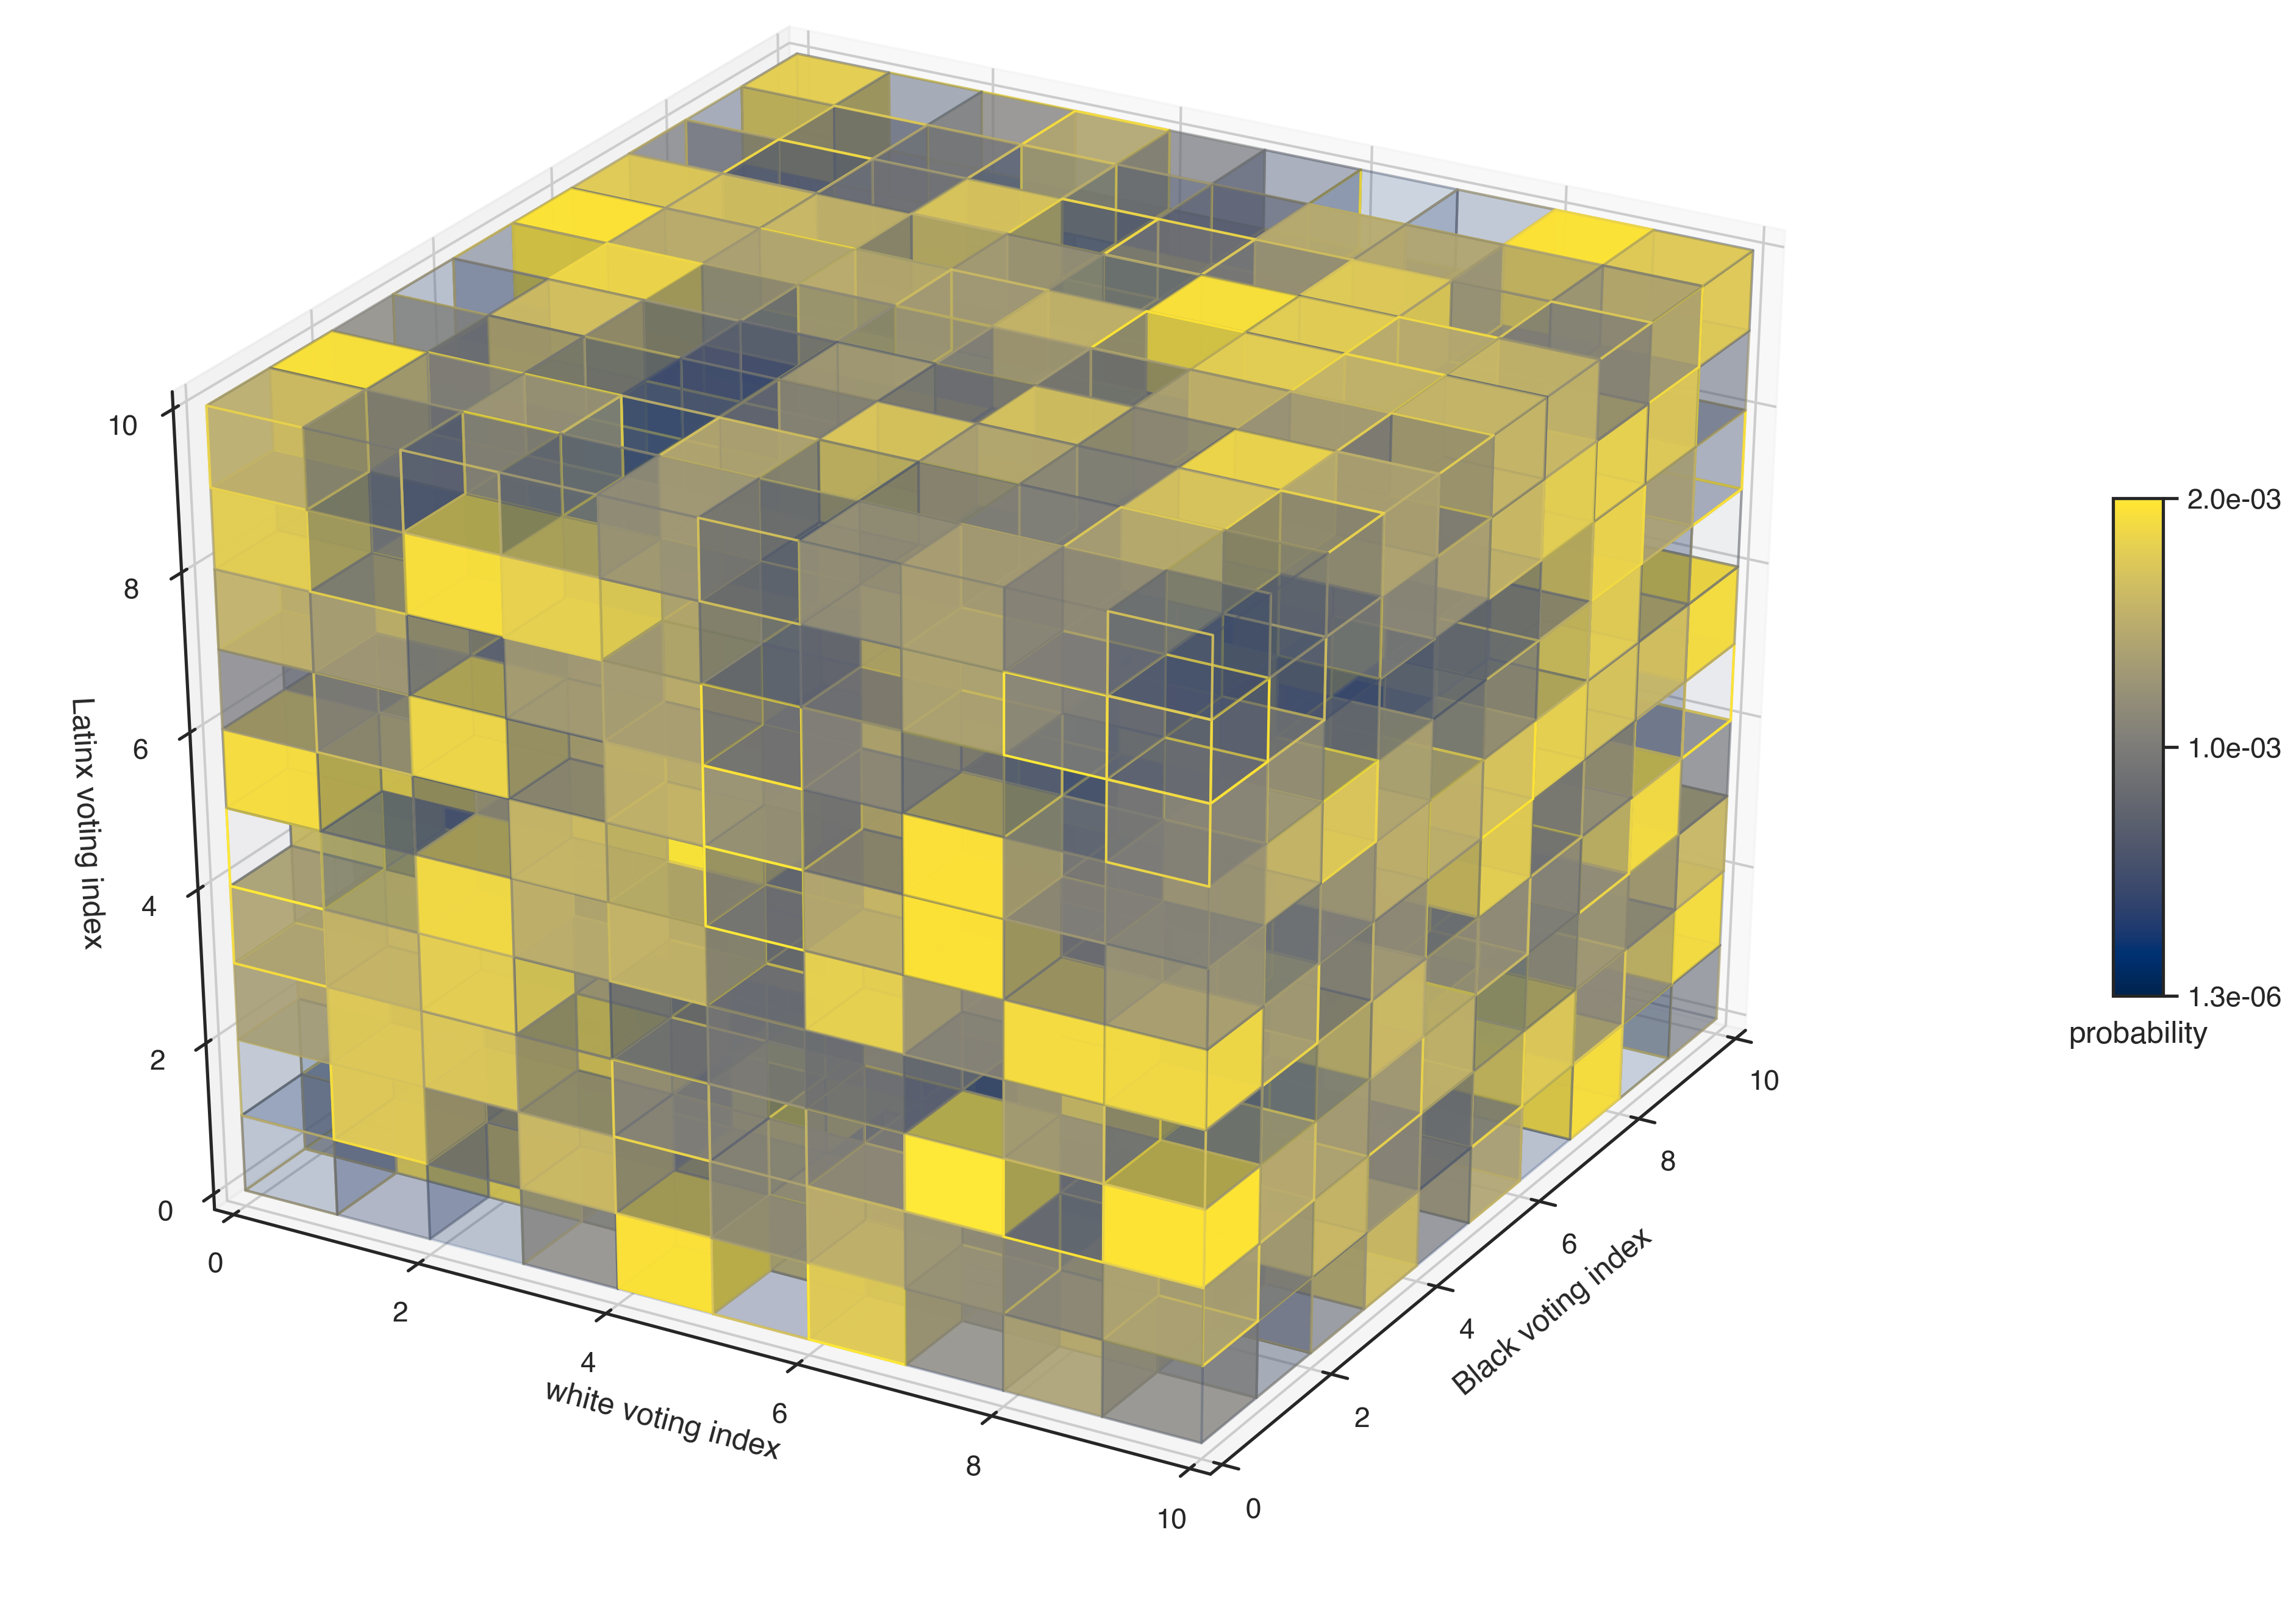
\includegraphics[width=\linewidth]{figures/3d_phc_plot_example.png}
 \caption{Example of a Rank $3$, Granularity $10$ Probabilistic Hypercube}
 \label{fig:3d_phc_plot_example}
\end{figure}

\begin{figure}[ht]\centering
 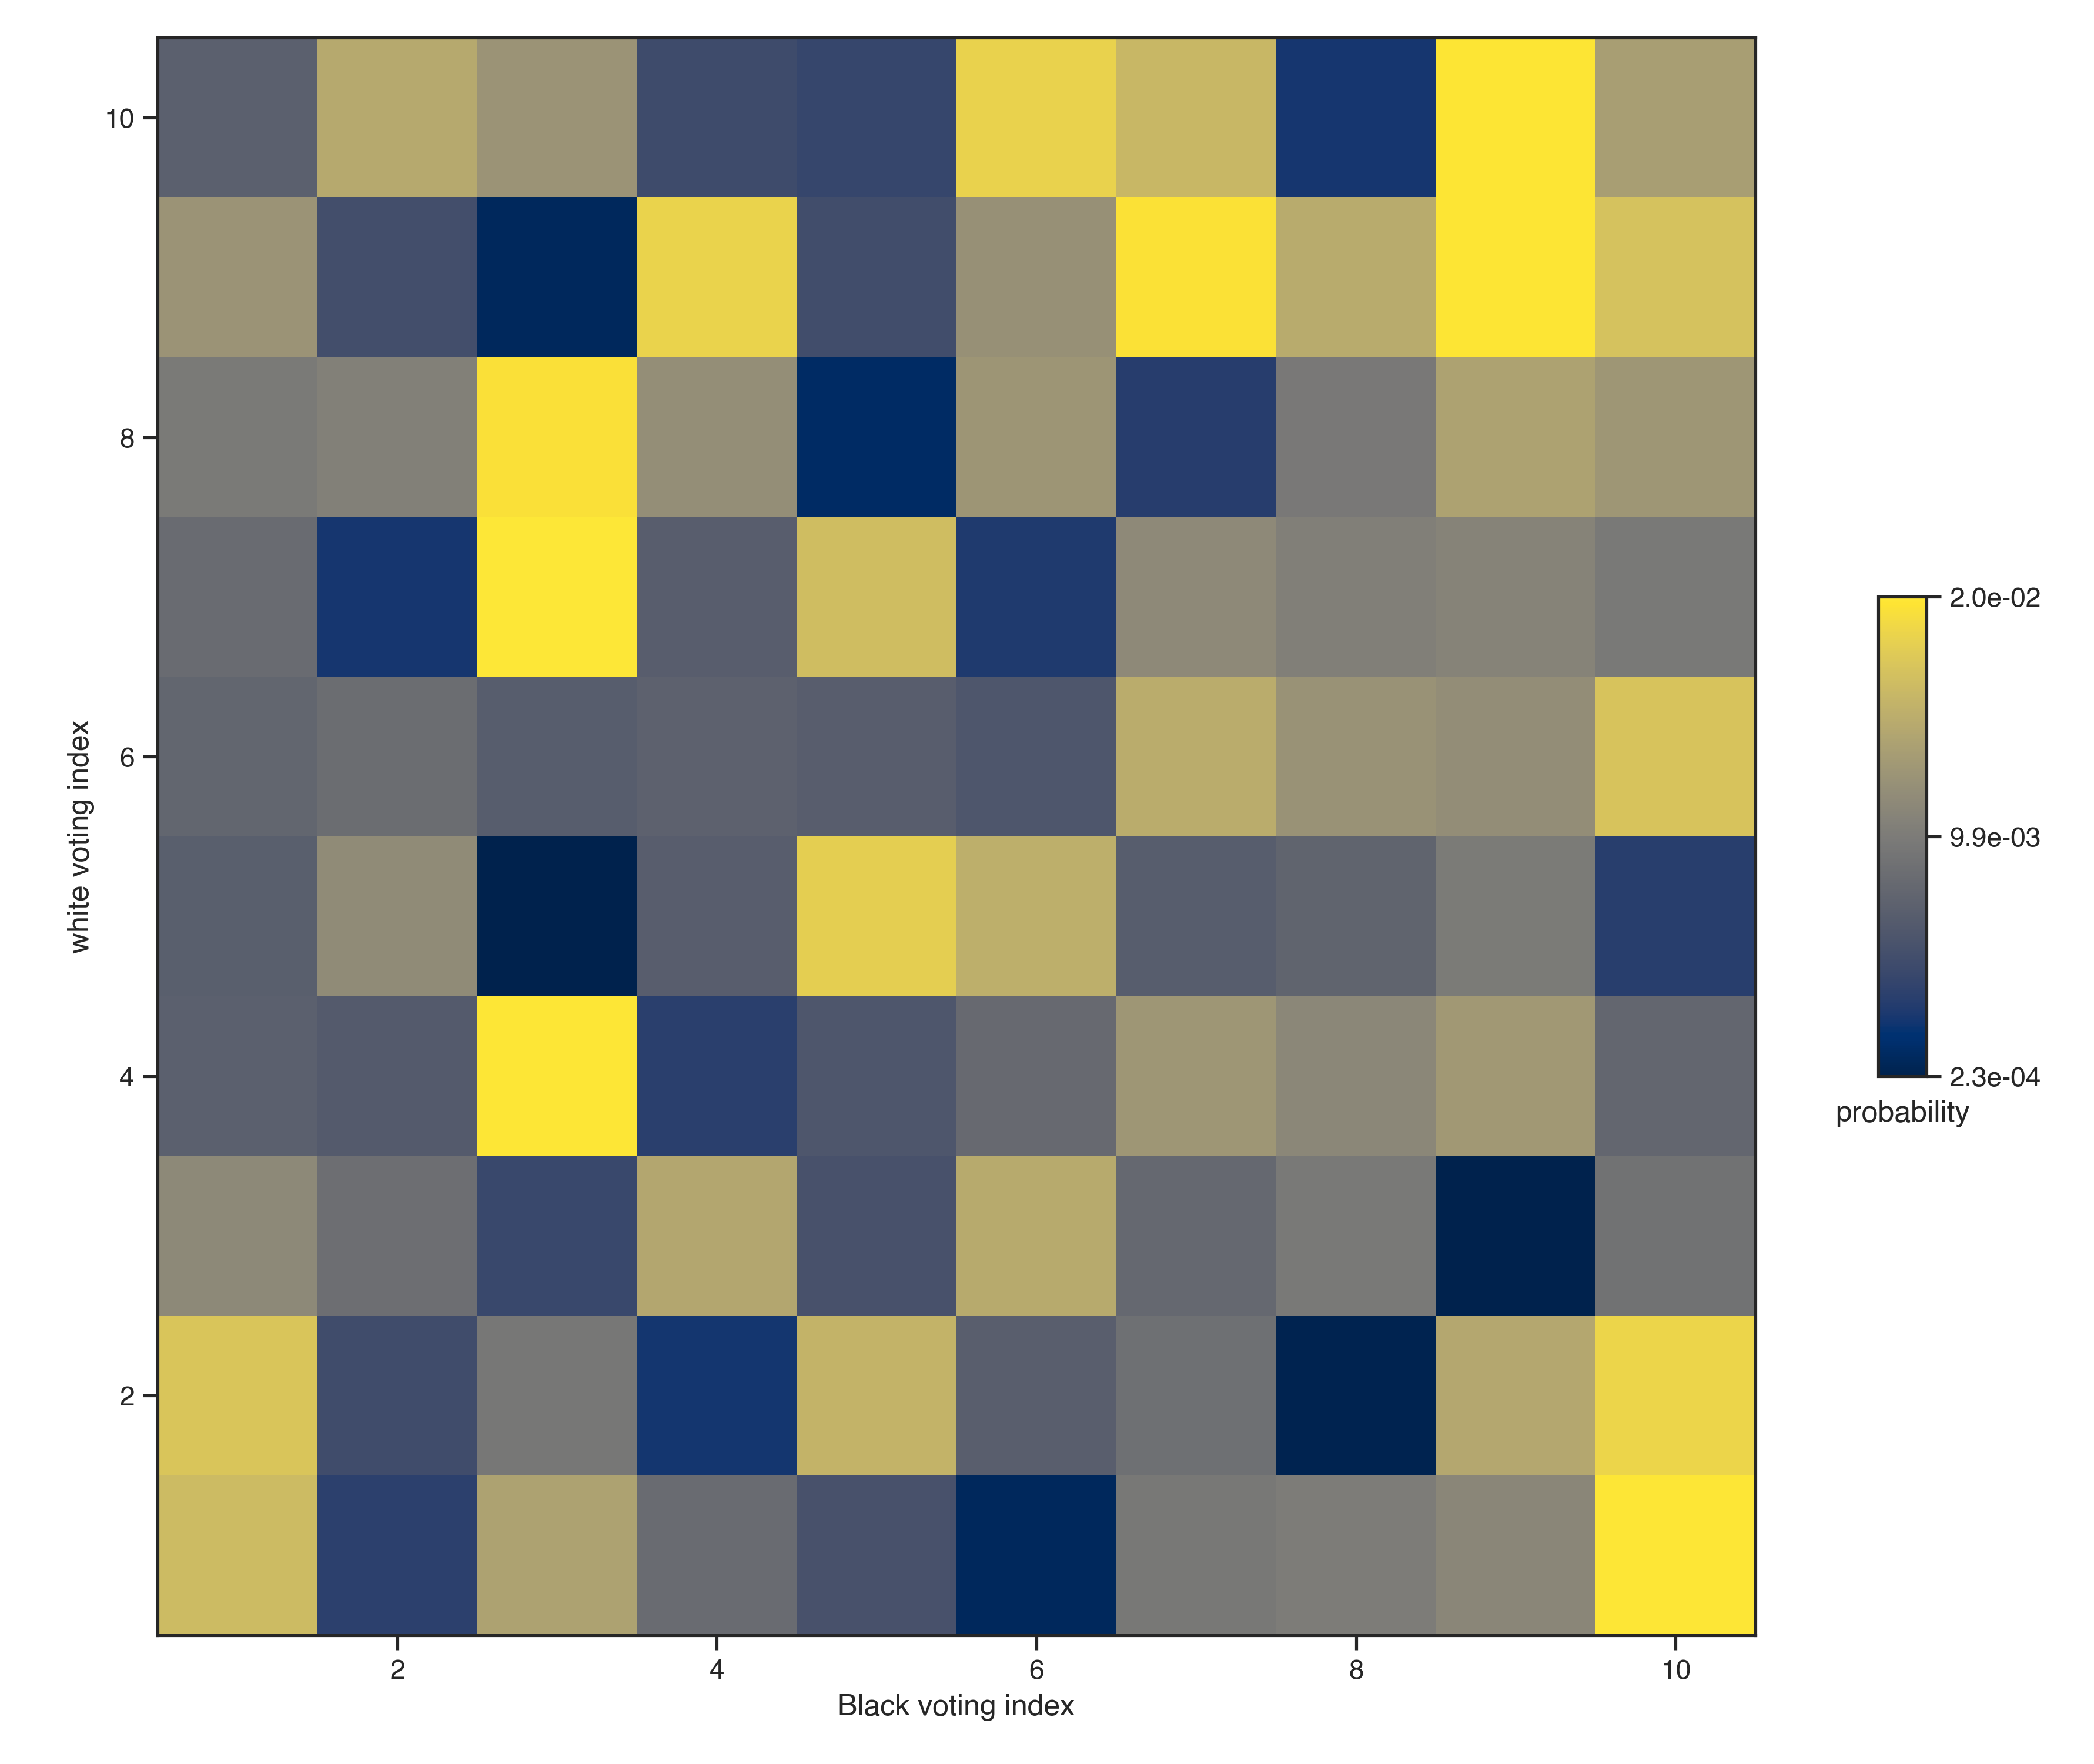
\includegraphics[width=\linewidth]{figures/2d_phc_plot_example.png}
 \caption{Example of a Rank $2$, Granularity $10$ Probabilistic Hypercube}
 \label{fig:2d_phc_plot_example}
\end{figure}

The rank $2$ case can also be visualized as a $3$-dimensional plot, where the third dimension is the probability associated with the cells of the PHC. Figure \ref{fig:2d_phc_plot_dist_example} illustrates this.

\begin{figure}[ht]\centering
 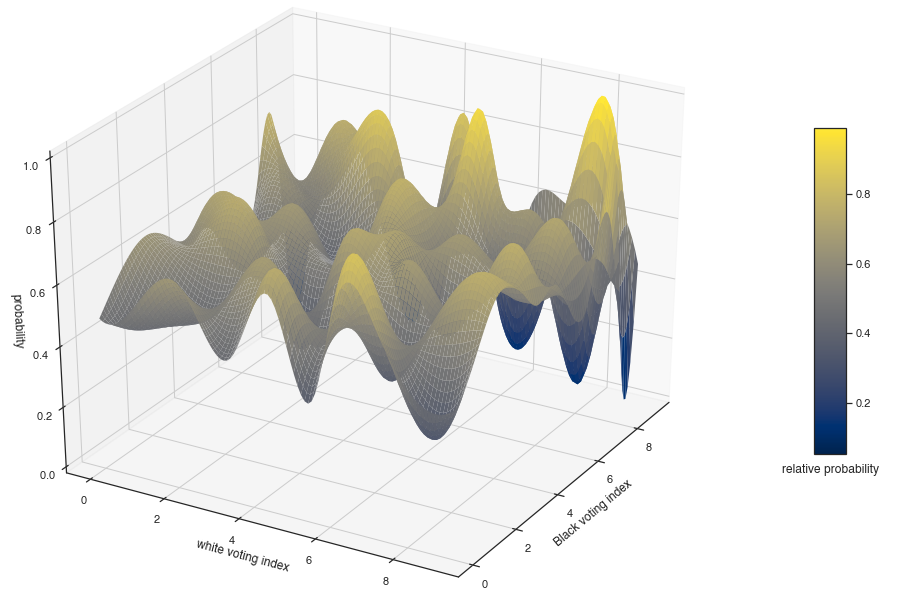
\includegraphics[width=\linewidth]{figures/2d_phc_plot_dist_example.png}
 \caption{The Probability Distribution within of a Rank $2$, Granularity $10$ Probabilistic Hypercube}
 \label{fig:2d_phc_plot_dist_example}
\end{figure}

Higher rank PHCs are difficult to visualize in similar ways, but the representational and intrinsic characteristics of the object remain the same. This is critical to the Discrete Voter Model's ability to generalize to arbitrarily diverse electorates, with arbitrarily precise demographic voting probabilities.


\section{expec\_votes}
\label{sec:ev}

\newthought{To be able to use probability hypercubes} as states in a Markov chain Monte Carlo method, the Discrete Voter Model employs two methods of determining how ``good" each PHC is. This determination, or scoring, is done with the modules \texttt{expec\_votes} and \texttt{prob\_votes}.

\texttt{expec\_votes} calculates the expectation for the vote outcome from a PHC, and compares that outcome to the observed electoral outcome. The closer they are, the higher the probability that this PHC represents a probable set of demographic voting probabilities for the given precinct.

Let there be some PHC with granularity $d$ representing $n$ demographic groups, for some cell at index $\{i_0, i_1, i_2, \dots, i_n\} = \left\{i_j\right\}_{j=0}^n$:

Let $i = 0, 1, \dots, m$ be the cells in the hypercube, where $m = d^n$.

Let $p_i$ be the probability of being in cell $i$.

Let $j = 0, 1, \dots, n$ be the demographic groups.

Let $q_j$ be the probability of demographic group $j$ to vote for the given candidate. ${q}_{j=0}^n =$ the demographic voting probabilities from Section \ref{sec:phc}.

Let $s_j$ be the population of demographic group $j$ in the precinct.

Let $v$ be the observed number of votes cast for the candidate in the precinct.

The expectation of a PHC is thus given by Equation \ref{eq:expec_votes}.

\begin{equation}
 \mathbb{E}(\text{PHC}) = \sum_{i = 0}^m p_i \left(\sum_{j = 0}^n q_j \cdot s_j\right)
 \label{eq:expec_votes}
\end{equation}

In addition to calculating the expectation of a PHC, the \texttt{expec\_votes} module compares that expectation to the observed electoral vote outcome in a precinct. It calculates the $L1$-norm of the difference between the two, then uses the function in Equation \ref{eq:asymptote} to convert it to a representation of the log-probability that the PHC has the same expectation as the vote outcome.

Let $x$ be the $L1$-norm of the difference between the expectation of a PHC and the electoral vote outcome, $v$:

$$x = \Vert \mathbb{E}(PHC) - v \Vert_1$$

\begin{equation}
  f(x) = \log\left(\frac{1}{x + 1}\right)
  \label{eq:asymptote}
\end{equation}

The more negative the value of $f(x)$, the less likely the PHC is to be able to generate the outcome of the election and be accepted in the Markov chain.


\section{prob\_votes}
\label{sec:pv}

\newthought{The Discrete Voter Model} also uses the \texttt{prob\_votes} module to score a probability hypercube. \texttt{prob\_votes} directly calculates the probability that a given hypercube produced the observed election outcome.

With the same notation as \texttt{expec\_votes} in Section \ref{sec:ev}, additionally:

Let $a_j$ be the number of people in demographic group $j$ that voted for the given candidate.

Equation \ref{eq:prob_votes} is the probability that a given hypercube produced a given election outcome.

\begin{equation}
 \mathbb{P}(\text{PHC} \rightarrow v) =\sum_{\forall a_j \text{ s.t. } \sum_{\forall j \in [0, n]} a_j = v} \left(\prod_{j = 0}^n q_j^{a_j} \cdot (1 - q_j)^{s_j - a_j}\right) \cdot \frac{v!}{\prod_{a_j}a_j!}
 \label{eq:prob_votes}
\end{equation}

Equation \ref{eq:prob_votes} uses the Binomial distribution to calculate the probability of members of different demographic groups voting together in a way to produce the desired outcome. This is extensible to any number of demographic groups and can be repeated for any number of candidates.

A crucial step in this process is generating sets of $\{a_j\}_{j=0}^n$ such that:

$$\sum_{\forall a_j \text{ s.t. } \sum_{\forall j \in [0, n]} a_j = v}$$

These sets are all possible partitions of the observed electoral outcome into the demographic groups. For example, if $10$ people voted for a candidate, and there are three demographic groups, $3$ possible partitions for the people who voted for the candidate are shown in Table \ref{table:partitions}.

\begin{table}[!h]
 \centering
 \caption{Partitions of $10$ votes among $3$ demographic groups}
 \label{table:partitions}
 \begin{tabular}{|c|c|c|c|}
   \toprule
    Partition & Group $1$ Votes & Group $2$ Votes & Group $3$ Votes \\\midrule
    $1$ & $4$ & $3$ & $3$  \\
    $2$ & $2$ & $0$ & $8$  \\
    $3$ & $2$ & $4$ & $4$  \\
    \bottomrule
 \end{tabular}
\end{table}

Integer partitioning can be computationally expensive. The time complexity of most algorithms for it is $O(v (log v))$, where $v$ is the vote outcome of an election. However, the Discrete Voter Model limits the size of partitions to be the number of demographic groups in the electorate, $n$. While DVM generalizes well to a large number of demographic groups, $n$ is unlikely to get large enough to make this integer partitioning step a time bottleneck. With that said, most algorithms for this process have space complexity $O(n^2)$. While limiting the size of partitions does reduce the space necessary, to further mitigate that use of space, DVM creates the set of integer partitions as a Python generator. Hence, values are treated like a stream, where computation is delayed until a partition is necessary, and the set of partitions is treated like a regular iterator. Finally, since integer partitions are used several times in the computation, and only depend on the vote outcome and the shape of the PHC, not the values in the PHC, the partitions can be generated once, and reused at every step in the MCMC method.

The full code for this partitioning process can be found in the appendix, either in the full repository or as Listing \ref{lst:integer_partition}.

The partitions are used to calculate the probability, as shown in Equation \ref{eq:prob_votes}. That probability is that of some candidate's and precinct's hypercube producing the observed electoral outcome. \texttt{prob\_votes} uses this to calculate the log-probability. The more negative that value, the less likely the PHC generated the outcome of the election and is accepted in the Markov chain. This scoring method is more intuitive and perhaps more precise, but it is much more computationally expensive. The calculations of large products, exponents, and especially factorials makes this much slower than scoring by expectation with \texttt{expec\_votes}.

\section{elect}
\label{sec:elect}

\newthought{The Discrete Voter Model} operates on data from elections, and the \texttt{elect} module prepares and packages the data for use.

This module implements the \texttt{Election} class, a data structure and accompanying methods that represents an election in a district. It has the following attributes:

\begin{enumerate}
  \item \texttt{candidates}: the candidates
  \item \texttt{dpp}: demographic distribution, per precinct
  \item \texttt{dvp}: the demographic voting probabilities, per precinct
  \item \texttt{mock}: whether the election is a mock election
  \item \texttt{name}: the name of the election
  \item \texttt{num\_demo\_groups}: the number of demographic groups in the district
  \item \texttt{outcome}: the vote outcome, by demographic group, of the election, per precinct
  \item \texttt{precincts}: the precinct IDs
  \item \texttt{vote\_totals}: the vote totals of each candidate, per precinct
  \item \texttt{winner}: the winner of the election
\end{enumerate}

An \texttt{Election} object for a mock election is initialized by providing the candidates, demographic distribution per precinct, and demographic voting probabilities (DVP) per precinct. Upon initialization, an election is simulated based on how each demographic votes, and other attributes, like the outcome, vote totals, and winner, are calculated.

That DVP is typically the desired result of the Discrete Voter Model, and by providing it to mock elections that then use it to generate election data, one can run the model on the object and attempt to recover the ``truth" that generated the results of the election. This is covered in depth in Section \ref{sec:eval}.

An \texttt{Election} object for a real election is initialized by providing the candidates, demographic distribution per precinct, and vote totals per precinct. Upon initialization, the election is ``decided" by calculating which of the candidates won.

The \texttt{elect} module also provides a function, \texttt{create\_elections}, that takes demographic data per precinct and voting data per precinct, both as the ubiquitous \texttt{Pandas DataFrame}s, to create an \texttt{Election} object. This allows DVM to be deployed quickly and easily to real election data. Section \ref{sec:eval} employs it for the case studies of North Carolina and Chicago.

The Discrete Voter Model uses an \texttt{Election} object's candidates, demographic distribution per precinct, and vote totals to create probabilistic hypercubes and run the Markov chain Monte Carlo method to find a distribution of PHCs that could have resulted in that \texttt{Election}'s outcomes. For mock elections, the accuracy of DVM can be compared to the original DVP that generated the \texttt{Election} object.


\section{dvm}
\label{sec:dvm}

\newthought{The final module}, and the one that runs the entire process, is \texttt{dvm}. It implements the Markov chain Monte Carlo method with Hamiltonian Monte Carlo (HMC) and Random Walk Metropolis (RWM) kernels, with both probability-based and expectation-based state scoring.

The Discrete Voter Model's MCMC method used probabilistic programming Python package \href{https://www.tensorflow.org/probability}{TensorFlow Probability} (TFP) as a substrate. TFP is a relatively new probabilistic programming package maintained by Google and the TensorFlow team. It is built on their popular open source machine learning platform, TensorFlow, and offers many advantages over a pure Python implementation of MCMC.\cite{tfp} The top three advantages to the Discrete Voter Model are:

\begin{enumerate}
  \item Nearly all of the operations are vectorized, allowing for much more efficient computation on high-dimensional objects like probabilistic hypercubes.
  \item It automatically scales to different platforms and architectures. Without any difference in the code, this allows the Discrete Voter Model to be able to be run on CPUs (central processing units) found in most computers, GPUs (graphics processing units) found in more powerful computers and sometimes optimized for machine learning, and TPUs (tensor processing units) developed by Google as AI accelerator application-specific integrated circuits (ASIC). As one increases the granularity of their PHC or the complexity of an election, they will be able to benefit from the increased computing power of modern machines.
  \item TensorFlow, and thus TensorFlow Probability, has lazy evaluation built in, through the \texttt{Graph} structure. TensorFlow \texttt{Graphs} employ the dataflow programming paradigm to increase the efficiency of parallel computations.\cite{tf_graph} This allows for:
  \begin{enumerate}
    \item easy identification and execution of operations that can be computed in parallel.
    \item distributed computing to take advantage of several machines at once.
    \item saving the model as a language-agnostic \texttt{Graph}. The \texttt{Graph} can then be executed in any of the many TensorFlow-compatible languages. For example, a graph generated in Python can be executed in C++.
    \item visualizing the \texttt{Graph} with built-in tools.
  \end{enumerate}
\end{enumerate}

Specifically, TFP is used to create the transition kernels and sample from the Markov chain.


The final subroutine, \texttt{mcmc}, runs the Markov chain Monte Carlo method with the Metropolis-Hastings algorithm, employing either \texttt{expec\_votes} or \texttt{prob\_votes} to score candidates.

The pseudocode for the MCMC is as follows:

\begin{enumerate}
  \item Choose a kernel: either Random Walk Metropolis or Hamiltonian Monte Carlo
  \item Choose a scoring function, $g$: either \texttt{expec\_votes} or \texttt{prob\_votes}
  \item Initialize some probabilistic with \texttt{phc}, $X_i$ where ${X}_{i=0}^t$ is the full sample. Score $X_i$ it with the kernel of choice to get $s_i$
  \item Iterate $t$ times. At each iteration, $i$:
  \begin{enumerate}[nolistsep]
    \item Generate a candidate hypercube, $Y_{i+1}$, with the kernel
    \item Calculate the score for that candidate, $s_{i+1} = g(Y_{i+1})$
    \item Accept $X_i$ with probability $\alpha = \frac{s_{i+1}}{s_i}$
    \begin{enumerate}[nolistsep]
      \item If accepted, $X_{i + 1} \leftarrow Y_{i + 1}$
      \item If rejected, $X_{i + 1} \leftarrow X_{i}$
    \end{enumerate}
  \end{enumerate}
  \item Burn a predetermined fraction of the observations at the beginning of the sample. Removing that early ``burn-in" period has been shown by some studies to be effective in creating a better sample.\cite{mcmc_methods}
  \item Output the sample as the distribution of probability hypercubes.
\end{enumerate}

The HMC kernel, \href{https://www.tensorflow.org/probability/api_docs/python/tfp/mcmc/HamiltonianMonteCarlo}{\texttt{tfp.mcmc.HamiltonianMonteCarlo}}, is initialized with an adaptive step size for the first $60\%$ of the burn-in period. The adaptive step size is controlled by \\\href{https://www.tensorflow.org/probability/api_docs/python/tfp/mcmc/SimpleStepSizeAdaptation}{\texttt{tfp.mcmc.SimpleStepSizeAdaptation}}, and is based on research by Andrieu and Thoms that shows that when the first few steps of an HMC-directed chain are allowed to adapt the step size towards the direction of the log probability of the state, the succeeding steps are more fruitful.\cite{hmc_adaptive}.

The RWM kernel, \href{https://www.tensorflow.org/probability/api_docs/python/tfp/mcmc/RandomWalkMetropolis}{\texttt{tfp.mcmc.RandomWalkMetropolis}}, is initialized with a proposal function that chooses two cells of the probability hypercube at random, and adds a small value, $\epsilon$, to one while subtracting it from the other. That proposal function is reversible and allows for good mixing, while also being simple enough to be performant.

Both kernels trace the log-probability and log-acceptance rate of the chain during sampling.

\texttt{dvm} implements the lower level functions for running the MCMC, \texttt{rwm} and \texttt{hmc}. It also implements the higher level function \texttt{dvm\_election} that applies the Discrete Voter Model to an \texttt{Election} object.

Finally, the module implements functions, \texttt{chain\_mle} and \texttt{mean\_phc}, for finding the Maximum Likelihood Estimate and the sample mean of distributions/samples produced by the model. These are quite useful when determining the central tendencies of the sample, and evaluating it easily.


\section{Evaluation}
\label{sec:eval}

\newthought{There are two auxiliary modules}, \texttt{dvm\_plot} and \texttt{dvm\_eval}, that provide visualizations and analysis of the Discrete Voter Model's results and behavior.

\texttt{dvm\_plot} provides a function to generate trace plots of the chains' results, as well as a bevy of functions to visualize the distribution of PHCs and the PHCs themselves. Those functions generated Figures \ref{fig:3d_phc_plot_example}, \ref{fig:2d_phc_plot_example}, and \ref{fig:2d_phc_plot_dist_example}.

All of the methods for inferring racially polarized voting noted in Chapter \ref{chap:background}, including ecological regression, homoegeneous precincts, and King's EI, are necessarily imperfect -- as is the Discrete Voter Model. The extent of that imperfection, however, can be evaluated and compared.

\texttt{dvm\_eval} is crucial to evaluating the Discrete Voter Model's performance generally, as well as how PHC granularity, the number of MCMC iterations, and kernel and score function choices interact with differences in election sizes and types to produce different results. Those results can be compared to the mock \texttt{Election} object's \texttt{dvp} attribute which generated the election's data. The \texttt{dvm\_evaluator} function does this comparison by running DVM and calculating the mean squared error (MSE), a common loss metric, between DVM's result and the \texttt{Election}'s DVP. The lower the MSE, the more accurate the model's predictions. \texttt{dvm\_evaluator} also records the time taken to run the Discrete Voter Model.

In addition, for the $2 \times 2$ case, \texttt{dvm\_eval} has the function \texttt{kei\_evaluator} that can similarly evaluate the performance of the canonical King's Ecological Inference method on mock elections. Those results can then be compared to the Discrete Voter Model's.

A set of experiments were created and run to determine the viability of the Discrete Voter Model. Those experiments' specifications and results are in \hyperref[chap:results]{Results}.
